\section{Network Server Configuration}

\subsection{Node definition}

The LoRaWAN end-node is registered within the ResIoT platform under the name \textbf{SN\_NODE\_J}. To ensure secure and unique connectivity within the network, the device is configured using the \gls{OTAA} method. Its primary identifiers include:

\begin{itemize}
    \item \textbf{Device EUI:} 7a:39:32:35:59:37:91:94.
    \item \textbf{Application EUI:} SEN\_NET\_2526.
    \item \textbf{Application KEY:} f3:1c:2e:8b:c6:71:28:1d:51:16:f0:8f:f0:b7:92:8f.
\end{itemize}

The node is set as a LoRaWAN Class A device, operating on the EU868 frequency band, which optimizes power consumption by only opening receiving windows after an uplink transmission. The internal data architecture of the node is organized through a series of \textbf{Node Fields} that act as the destination for the decoded payload values, defined in \autoref{tab:node_fields}.

\begin{table}[h]
    \centering
    \caption{Node Field Definitions for SN\_NODE\_J}
    \label{tab:node_fields}
    \begin{tabular}{|l|l|l|}
        \hline
        \textbf{Field Tag} & \textbf{Label} & \textbf{Content Type} \\ \hline
        Latitude & Latitude & Numeric \\ \hline
        Longitude & Longitude & Numeric \\ \hline
        Altitude & Altitude & Numeric \\ \hline
        Light & Light & Numeric \\ \hline
        Temperature & Temperature & Numeric \\ \hline
        Humidity & Humidity & Numeric \\ \hline
        Time & Time & String \\ \hline
        Sats & Sats & Numeric \\ \hline
        Moisture & Moisture & Numeric \\ \hline
        Red / Green / Blue & R / G / B & Numeric \\ \hline
        X / Y / Z & X / Y / Z & Numeric \\ \hline
    \end{tabular}
\end{table}

\subsection{LUA Scripting}

The data transmitted by the LoRaWAN end-node is received by the ResIoT platform as a hexadecimal payload. To make this information actionable, a LUA script is implemented to decode the raw byte array into human-readable sensor values. The script is structured into three main functional blocks:

\begin{itemize}
    \item \textbf{Binary Conversion Logic:} Since LoRaWAN payloads are optimized for low bandwidth, data is sent in binary format. The function \texttt{bytesToInt} handles Little Endian conversion. It reconstructs integers by iterating through the byte array and applying the formula:
    \begin{equation}
        Value = \sum_{i=0}^{size-1} bytes[start + i] \cdot 256^i
    \end{equation}
    It also includes logic to handle signed integers using Two's Complement verification.

    \item \textbf{Payload Decapsulation:} The \texttt{parsePayload} function slices the buffer to extract specific sensor variables based on predefined offsets:
    \begin{itemize}
        \item \textbf{GPS Coordinates:} Latitude and longitude are extracted as 4-byte signed integers and scaled by $10^{-6}$ to retrieve decimal degrees.
        \item \textbf{Environmental Sensors:} Temperature and humidity are decoded and scaled by $100.0$, while Light and Moisture use a $10.0$ divisor to restore their original floating-point precision.
        \item \textbf{Inertial Data:} Accelerometer values (X, Y, Z) are treated as 8-bit signed integers (\textit{int8}) to detect orientation and movement.
    \end{itemize}

    \item \textbf{Platform Integration:} After decoding, the script utilizes the \texttt{resiot\_setnodevalue} function. This updates the digital twin of the device within the platform, mapping the decoded variables (e.g., \textit{Temperature, Latitude, Red}) to specific nodes for real-time visualization and storage.
\end{itemize}

The script also includes an \texttt{Origin} check, allowing for manual testing with a static hex string or automatic processing when a live uplink is detected from the LoRaWAN gateway.

\begin{lstlisting}[language=lua, caption={LUA Scripting - SN\_TEST\_J}]
    -- Helper function to convert bytes to Integer (Little Endian)
    function bytesToInt(bytes, start, size, signed)
        local val = 0
        for i = 0, size - 1 do
            val = val + (bytes[start + i] * (256 ^ i))
        end
        if signed and val >= (256 ^ size) / 2 then
            val = val - (256 ^ size)
        end
        return val
    end

    function parsePayload(appeui, deveui, payload)
        -- Convert hex payload to byte array
        local bytes = resiot_hexdecode(payload)

        -- 1. GPS Data (1 to 17)
        local lat  = bytesToInt(bytes, 1, 4, true) / 1000000.0
        local lon  = bytesToInt(bytes, 5, 4, true) / 1000000.0
        local alt  = bytesToInt(bytes, 9, 4, true) / 100.0 

        -- GPS Time (13-15) HHMMSS
        local hh = bytes[13]
        local mm = bytes[14]
        local ss = bytes[15]
        local time = string.format("%02d:%02d:%02d", hh, mm, ss)

        local sats = bytes[16]                            

        -- 2. Temperature and Humidity Data (17 to 20)
        local temp = bytesToInt(bytes, 17, 2, true) / 100.0
        local hum  = bytesToInt(bytes, 19, 2, false) / 100.0

        -- 3. Brightness and Moisture (21 to 24)
        local light    = bytesToInt(bytes, 21, 2, false) / 10.0
        local moisture = bytesToInt(bytes, 23, 2, false) / 10.0

        -- 4. Color RGB (Offsets 25 to 27)
        local r = bytes[25]
        local g = bytes[26]
        local b = bytes[27]

        -- 5. Accelerometer (28 to 30)
        -- These are int8 (signed). If value > 127, it's negative.
        local function toInt8(b) return b > 127 and b - 256 or b end
        local x = toInt8(bytes[28]) / 10.0
        local y = toInt8(bytes[29]) / 10.0
        local z = toInt8(bytes[30]) / 10.0

        -- Debug Logs
        resiot_debug(string.format("GPS: Lat: %.6f, Long: %.6f, Alt: %.2f, Time: %s, Sats: %d", lat, lon, alt, time, sats))
        resiot_debug(string.format("Sensors: Temp: %.2f, Hum: %.2f, Light: %.1f, Moisture: %.1f", temp, hum, light, moisture))
        resiot_debug(string.format("Color: R:%d, G:%d, B:%d", r, g, b))
        resiot_debug(string.format("Accel: X:%.1f, Y:%.1f, Z:%.1f", x, y, z))

        -- Update Nodes in ResIoT
        resiot_setnodevalue(appeui, deveui, "Latitude", lat)
        resiot_setnodevalue(appeui, deveui, "Longitude", lon)
        resiot_setnodevalue(appeui, deveui, "Altitude", alt)
        resiot_setnodevalue(appeui, deveui, "Time", time)
        resiot_setnodevalue(appeui, deveui, "Sats", sats)
        resiot_setnodevalue(appeui, deveui, "Temperature", temp)
        resiot_setnodevalue(appeui, deveui, "Humidity", hum)
        resiot_setnodevalue(appeui, deveui, "Light", light)
        resiot_setnodevalue(appeui, deveui, "Moisture", moisture)
        resiot_setnodevalue(appeui, deveui, "Red", r)
        resiot_setnodevalue(appeui, deveui, "Green", g)
        resiot_setnodevalue(appeui, deveui, "Blue", b)
        resiot_setnodevalue(appeui, deveui, "X", x)
        resiot_setnodevalue(appeui, deveui, "Y", y)
        resiot_setnodevalue(appeui, deveui, "Z", z)
    end

    -- --- Main Process ---
    Origin = resiot_startfrom()

    if Origin == "Manual" then
        -- Test payload (14 bytes hex)
        payload = "0A00FE3E2102996E2E08E808E813" 
        appeui = "70b3d57ed000fc4d"
        deveui = "7a39323559379194"
    else
        appeui = resiot_comm_getparam("appeui")
        deveui = resiot_comm_getparam("deveui")
        payload, err = resiot_getlastpayload(appeui, deveui)
    end

    parsePayload(appeui, deveui, payload)
\end{lstlisting}

The LUA script is integrated into the ResIoT ecosystem through the LoRaWAN node's automation logic. Rather than running as a static process, the code is embedded within the \textbf{On RX} (On Receive) event. This configuration establishes an event-driven architecture where the script remains idle until a new radio frame is successfully demodulated by the gateway and forwarded to the network server.

\begin{figure}[H]
    \centering
    \includegraphics[width=1\textwidth]{images/scene.png}
    \caption{ResIoT Node Automation - On RX Event}
    \label{fig:scene}
\end{figure}

Once an uplink packet is received, the platform automatically triggers the execution of the script, passing the device identifiers and the raw hexadecimal payload as input parameters. This seamless execution allows the system to act as a real-time middleware, transforming binary data into structured information.

\subsection{Dashboard}

The monitoring interface is organized within a dedicated group named \textbf{SN\_GROUP\_J}. The dashboard consists of a variety of widgets designed to provide real-time telemetry, spatial data, and historical trends. The following list details the specific widgets and their respective visualization types:

\begin{itemize}
    \item \textbf{Node J - Temperature / Humidity / Brightness / Soil Moisture:} These environmental parameters are displayed using \textbf{Gauge} widgets, providing an intuitive immediate-view of current levels.
    \item \textbf{Node J - Historical Values:} A \textbf{Line Chart} is dedicated to tracking the temporal evolution of sensor data over time.
    \item \textbf{Node J - Alarms:} A \textbf{Table Values} widget is configured to show the status of the boolean alarm flags, allowing for quick identification of threshold breaches (Temperature / Humidity / Brightness / Soil Moisture).
    \item \textbf{Node J - Leaf Color:} The RGB values extracted from the sensor are represented through a \textbf{Pie} chart widget to visualize color composition.
    \item \textbf{Node J - Acceleration ($m/s^2$):} Motion and orientation data from the three-axis accelerometer are visualized using a \textbf{Line Chart}.
    \item \textbf{Node J - Location:} A \textbf{Maps} widget is utilized to track the GPS coordinates (\textit{Latitude} and \textit{Longitude}) decoded from the device payload.
\end{itemize}

\begin{figure}[H]
    \centering
    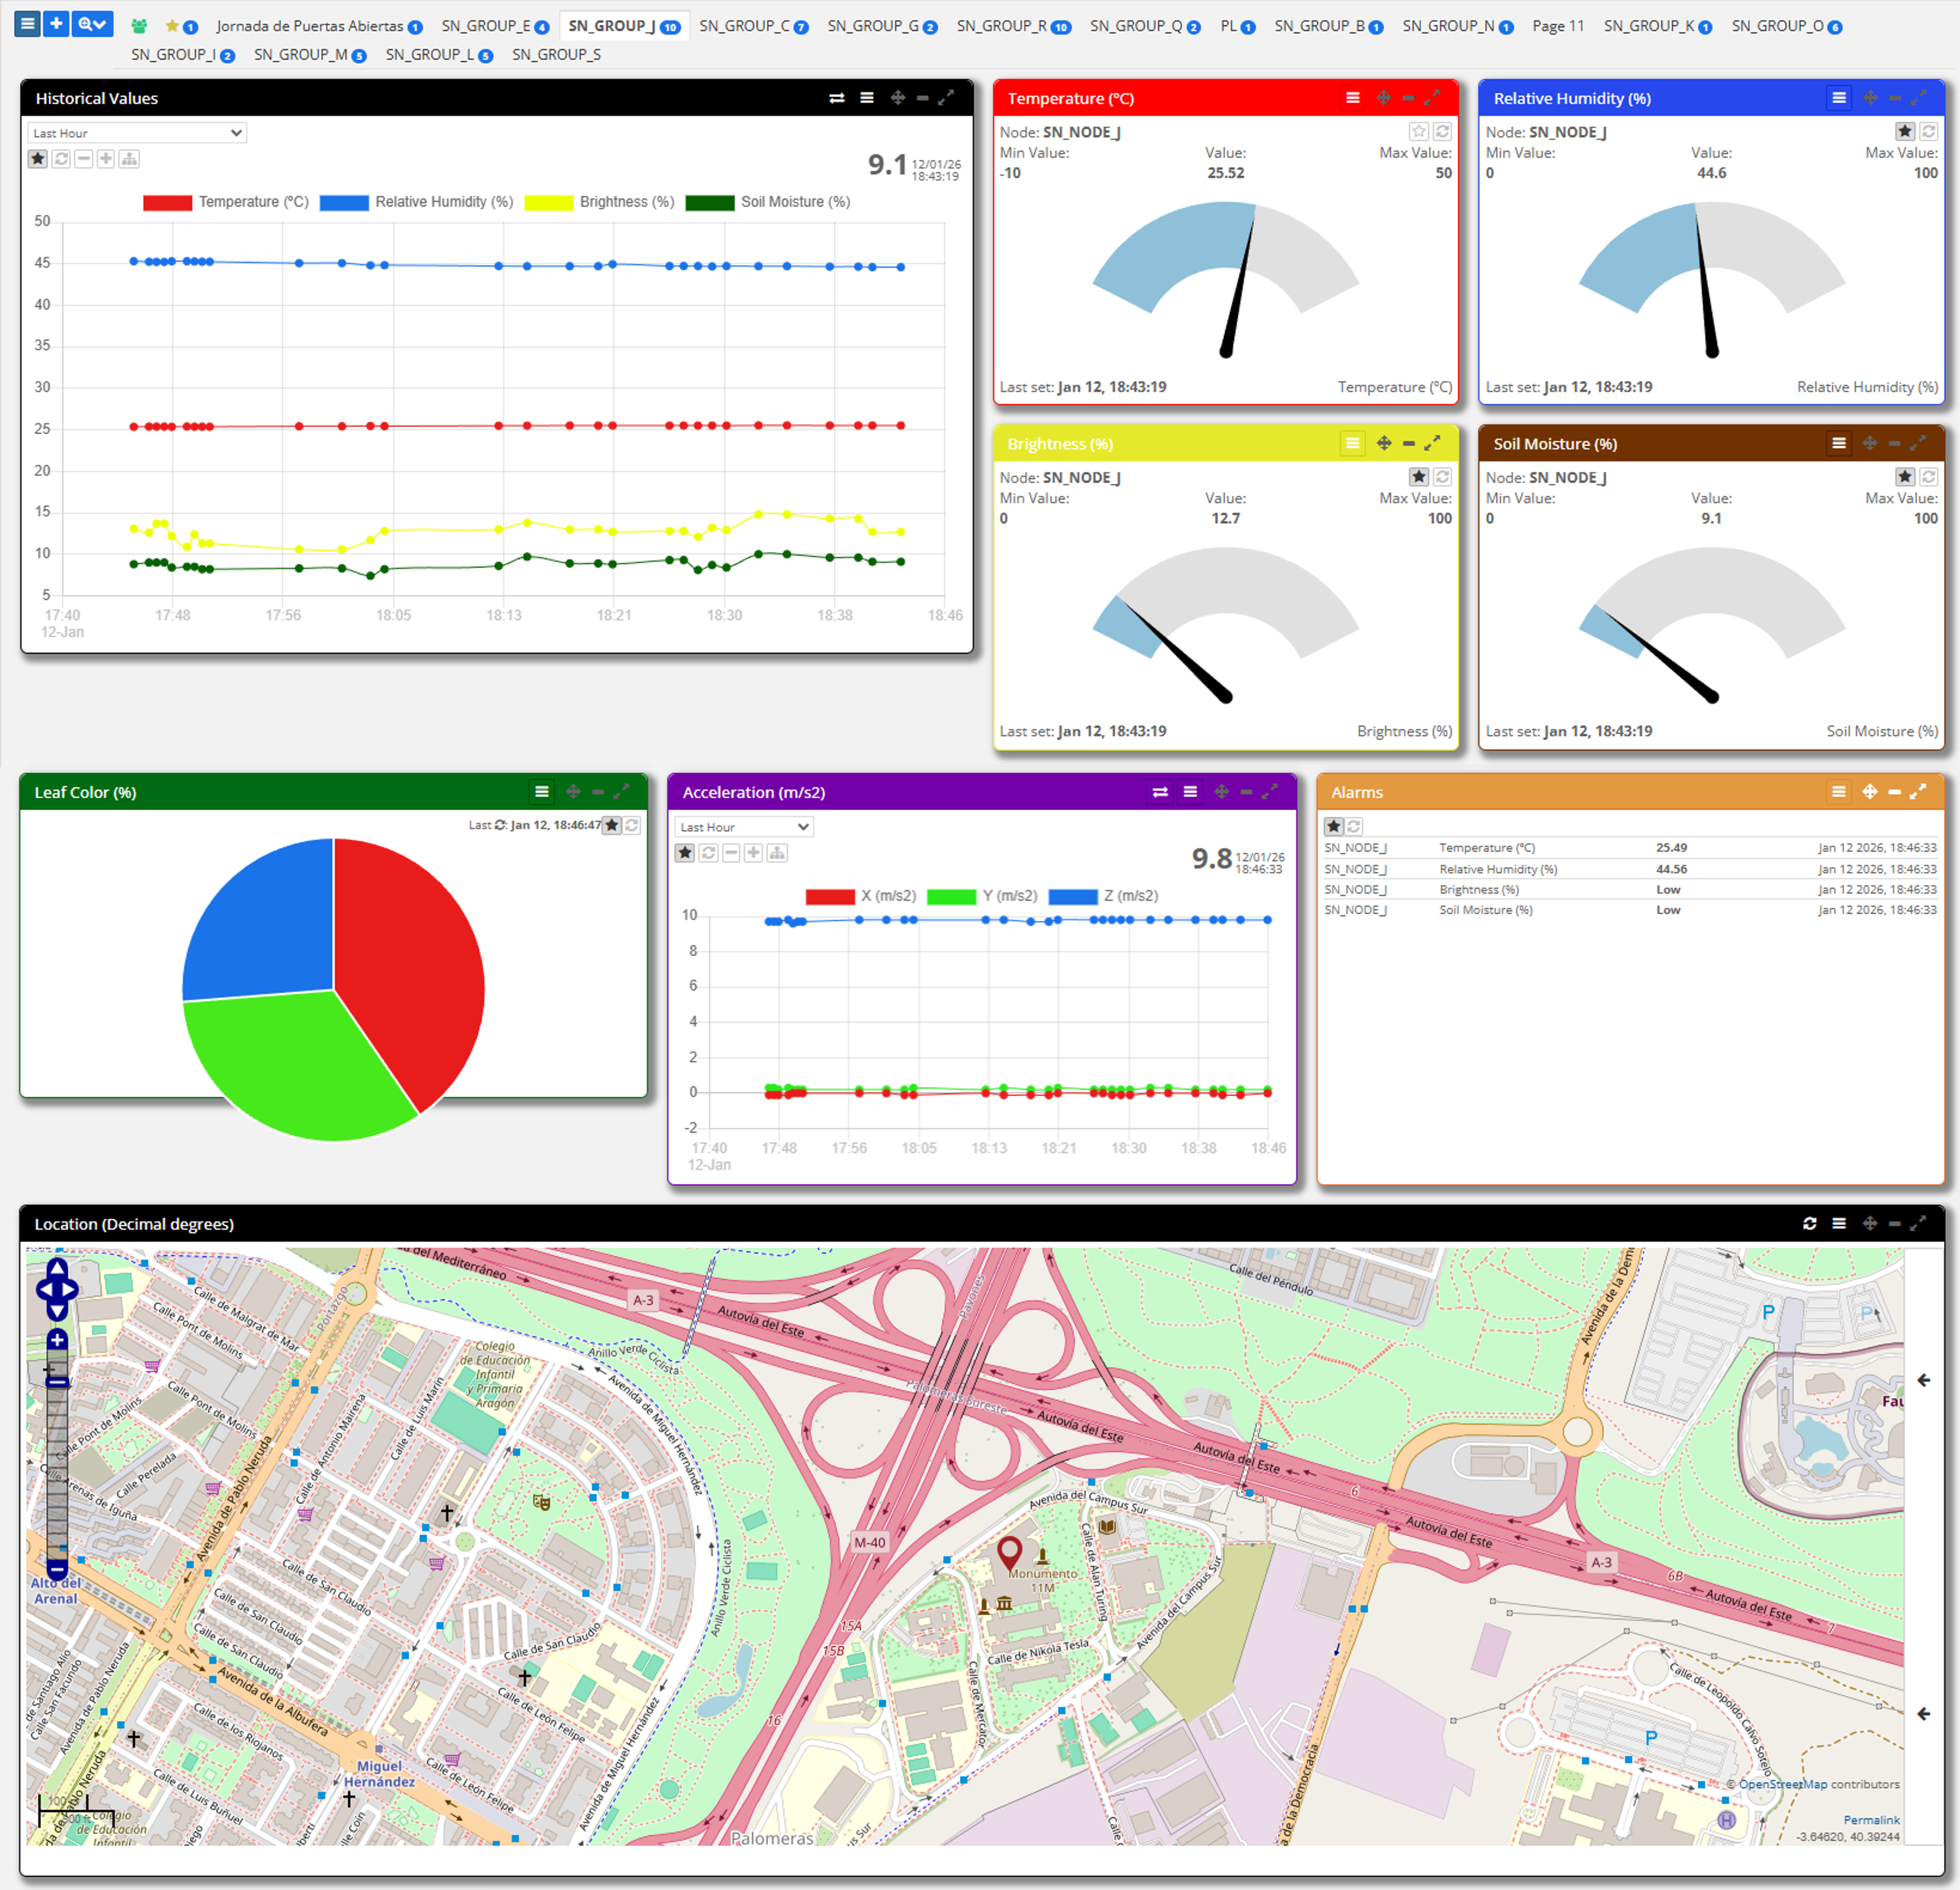
\includegraphics[width=1\textwidth]{images/dashboard.png}
    \caption{ResIoT Dashboard - SN\_GROUP\_J}
    \label{fig:dashboard}
\end{figure}

Each widget is set to \textbf{Visible} and is manually arranged to optimize the user experience within the platform's control panel. The gauges and charts pull data directly from the \textbf{Node Fields} updated by the LUA script during the \textit{On RX} automation event.

\subsubsection{Temperature / Humidity / Brightness / Soil Moisture Gauges}

The primary environmental metrics are visualized through four specialized \textbf{Gauge} widgets. These provide an immediate, high-visibility status of the sensors' current state within the \textbf{SN\_GROUP\_J} dashboard.

The configuration for these gauges (as exemplified by the Temperature widget in Figure \ref{fig:gauge_conf}) is defined by the following parameters:

\begin{itemize}
    \item \textbf{Data Mapping:} Each widget is linked to the specific numeric \textit{Node Field} updated by the LUA script (e.g., \texttt{Temperature}, \texttt{Humidity}, \texttt{Light}, or \texttt{Moisture}).
    \item \textbf{Range Calibration:} To provide context to the raw data, specific minimum and maximum thresholds are established:
    \begin{itemize}
        \item \textbf{Temperature:} Set from \textbf{-10°C} to \textbf{50°C}.
        \item \textbf{Humidity / Brightness / Soil Moisture:} Calibrated on a percentage scale from \textbf{0\%} to \textbf{100\%}.
    \end{itemize}
    \item \textbf{Visual Styling:} Each gauge utilizes a distinct header color (Red for Temperature, Blue for Humidity, Yellow for Brightness, and Brown for Soil Moisture) to facilitate rapid identification of the data source.
    \item \textbf{Unit Management:} The widgets are configured with their respective Units of Measurement (UM), such as \textbf{Celsius} for temperature, ensuring that the displayed value ($V$) is correctly interpreted by the user.
\end{itemize}

\begin{figure}[H]
    \centering
    \includegraphics[width=1\textwidth]{images/gauge_temp.png}
    \caption{Gauge Configuration - Temperature Example}
    \label{fig:gauge_conf}
\end{figure}

As shown in Figure \ref{fig:gauges}, the gauges also display the timestamp of the last received data packet (\textit{"Last set"}), confirming the real-time nature of the \textbf{On RX} automation process.

\begin{figure}[H]
    \centering
    \includegraphics[width=1\textwidth]{images/gauges.png}
    \caption{ResIoT Dashboard - Temperature / Humidity / Brightness / Soil Moisture Gauges}
    \label{fig:gauges}
\end{figure}

\subsubsection{Historical Values}

The \textbf{Node J - Historical Values} widget is a multi-variable \textbf{Line Chart} designed to monitor the temporal evolution of the environment. This visualization is crucial for identifying patterns, such as the correlation between temperature rises and humidity drops, or the impact of light intensity on soil moisture evaporation.

\begin{figure}[H]
    \centering
    \includegraphics[width=1\textwidth]{images/historical.png}
    \caption{ResIoT Dashboard - Historical Values Line Chart}
    \label{fig:historical}
\end{figure}

The configuration of this chart, as illustrated in Figure \ref{fig:hist_conf}, is based on the following technical parameters:

\begin{itemize}
    \item \textbf{Data Aggregation:} The chart simultaneously plots four distinct data series from the \texttt{SN\_NODE\_J} node fields: \textit{Temperature}, \textit{Relative Humidity}, \textit{Brightness}, and \textit{Soil Moisture}.
    \item \textbf{Color Coding:} To ensure visual consistency with the gauges, specific colors are assigned to each variable: Red for Temperature, Blue for Humidity, Yellow for Brightness, and Dark Green for Soil Moisture.
    \item \textbf{Time Window:} The widget is configured with a \textbf{Last Hour} default interval, providing a granular view of recent sensor activity.
    \item \textbf{Dynamic Scaling:} The Y-axis automatically adjusts to the numeric range of the incoming data, while the X-axis represents the chronological timeline updated in real-time by the \textit{On RX} automation.
\end{itemize}

\begin{figure}[H]
    \centering
    \includegraphics[width=1\textwidth]{images/historical_conf.png}
    \caption{Line Chart Configuration}
    \label{fig:hist_conf}
\end{figure}


\subsubsection{Alarms}

The \textbf{Alarms} widget is implemented as a \textbf{Table Values} display, providing a centralized view of the health status of all environmental sensors. Unlike the gauges, which show raw numerical data, this table is specifically configured to interpret threshold breaches and translate them into human-readable alerts.

As illustrated in the configuration details in Figure \ref{fig:alarms_conf}, the widget utilizes a conditional string replacement logic to define the status of each variable:

\begin{itemize}
    \item \textbf{Temperature Logic:} The system monitors for extreme conditions, displaying \textbf{"High"} if the value exceeds $50$ and \textbf{"Low"} if it falls below $-10$.
    \item \textbf{Environmental Thresholds:} For \textit{Relative Humidity}, \textit{Brightness}, and \textit{Soil Moisture}, a unified logic is applied where values above $75$ trigger a \textbf{"High"} status and values below $25$ trigger a \textbf{"Low"} status.
    \item \textbf{Real-time Monitoring:} If the current values are within the safe operational range (e.g., Temperature at $25.52$ or Humidity at $44.6$ as seen in Figure \ref{fig:alarms}), the table displays the actual numerical value.
    \item \textbf{Data Synchronization:} Every entry in the table is accompanied by a timestamp (\textit{"Date Last Setting"}), ensuring that the alerts correspond to the most recent LoRaWAN uplink processed by the \textit{On RX} automation.
\end{itemize}

\begin{figure}[H]
    \centering
    \includegraphics[width=1\textwidth]{images/alarms_conf.png}
    \caption{Table Configuration}
    \label{fig:alarms_conf}
\end{figure}

This visual organization allows the operator to instantly identify which specific sensor requires attention without having to manually analyze individual charts or gauges.

\begin{figure}[H]
    \centering
    \includegraphics[width=1\textwidth]{images/alarms.png}
    \caption{ResIoT Dashboard - Alarms Table}
    \label{fig:alarms}
\end{figure}

\subsubsection{Leaf Color}

The \textbf{Node J - Leaf Color} widget provides a qualitative representation of sensor data using a \textbf{Pie Chart} format. This visualization is specifically designed to display the relative distribution of the RGB color components decoded from the sensor payload.

The configuration of this widget, as detailed in Figure \ref{fig:color_conf}, includes the following parameters:

\begin{itemize}
    \item \textbf{Data Integration:} The chart aggregates three specific numeric \textit{Node Fields}: \textbf{Red}, \textbf{Green}, and \textbf{Blue}.
    \item \textbf{Visual Mapping:} To ensure an intuitive interpretation, each data element is assigned a representative color: Red for the Red (\%) field, Green for the Green (\%) field, and Blue for the Blue (\%) field.
    \item \textbf{Interactive Display:} The widget is configured to show specific values upon user interaction; for example, Figure \ref{fig:color} demonstrates a detected \textbf{Red} component of \textbf{41\%}.
    \item \textbf{Refresh Logic:} The chart includes an \textbf{Autorefresh} feature with a set interval of \textbf{30 seconds}, ensuring the visualization remains synchronized with the latest environmental data processed by the platform.
\end{itemize}

\begin{figure}[H]
    \centering
    \includegraphics[width=1\textwidth]{images/color_conf.png}
    \caption{Pie Chart Configuration}
    \label{fig:color_conf}
\end{figure}

By utilizing a circular proportional representation, the dashboard allows for an immediate assessment of color dominance, which can be critical for monitoring plant health or specific environmental light conditions.

\begin{figure}[H]
    \centering
    \includegraphics[width=1\textwidth]{images/color.png}
    \caption{ResIoT Dashboard - Leaf Color Pie Chart}
    \label{fig:color}
\end{figure}


\subsubsection{Acceleration}

\subsubsection{Location}

